\documentclass[]{article}
\usepackage{lmodern}
\usepackage{amssymb,amsmath}
\usepackage{dsfont}
\usepackage{graphicx}
\usepackage{ifxetex,ifluatex}
\usepackage{fixltx2e} % provides \textsubscript
\ifnum 0\ifxetex 1\fi\ifluatex 1\fi=0 % if pdftex
  \usepackage[T1]{fontenc}
  \usepackage[utf8]{inputenc}
\else % if luatex or xelatex
  \ifxetex
    \usepackage{mathspec}
  \else
    \usepackage{fontspec}
  \fi
  \defaultfontfeatures{Ligatures=TeX,Scale=MatchLowercase}
\fi
% use upquote if available, for straight quotes in verbatim environments
\IfFileExists{upquote.sty}{\usepackage{upquote}}{}
% use microtype if available
\IfFileExists{microtype.sty}{%
\usepackage[]{microtype}
\UseMicrotypeSet[protrusion]{basicmath} % disable protrusion for tt fonts
}{}
\PassOptionsToPackage{hyphens}{url} % url is loaded by hyperref
\usepackage[unicode=true]{hyperref}
\hypersetup{
            pdfborder={0 0 0},
            breaklinks=true}
\urlstyle{same}  % don't use monospace font for urls
\IfFileExists{parskip.sty}{%
\usepackage{parskip}
}{% else
\setlength{\parindent}{0pt}
\setlength{\parskip}{6pt plus 2pt minus 1pt}
}
\setlength{\emergencystretch}{3em}  % prevent overfull lines
\providecommand{\tightlist}{%
  \setlength{\itemsep}{0pt}\setlength{\parskip}{0pt}}
\setcounter{secnumdepth}{0}
% Redefines (sub)paragraphs to behave more like sections
\ifx\paragraph\undefined\else
\let\oldparagraph\paragraph
\renewcommand{\paragraph}[1]{\oldparagraph{#1}\mbox{}}
\fi
\ifx\subparagraph\undefined\else
\let\oldsubparagraph\subparagraph
\renewcommand{\subparagraph}[1]{\oldsubparagraph{#1}\mbox{}}
\fi

% set default figure placement to htbp
\makeatletter
\def\fps@figure{htbp}
\makeatother


\def\doubleunderline#1{\underline{\underline{#1}}}

\date{}

\usepackage{tcolorbox}

\begin{document}

\section{Lezione 1 - Stat model}\label{lezione-1---stat-model}

\subsubsection{5-03-2018}\label{section}

\emph{prof. Vittadini}

Intro: Il corso comprende 3 argomenti: + modello lineare classico e
estensione + modello lineare multivariato + applicazione di questo
modello su dati gerarchici

Lezioni teoriche (con approccio pratico) e laboratori (SAS e R) + tutor
(daniele.riggi@gmail.com).

Esame: 2 domande teoriche tra 15 preordinate (bastano le slide,
possibilità di approfondire sui libri indicati). Esercizio da svolgere
in classe o con SAS o con R.

Lezio: 1. Descrizione delle variabili e metriche. 2. Pulizia dei dati.
3. Statistiche descrittive: media, mediana, primo e terzo quantile, min
e max, matrice di correlazione (eliminare variabili fortemente
correlate, in quanto possono avere un'influenza negativa sul modello),
scatter plot. 4. Costruzione di un modello statistico.

Quali sono gli indici che mi dicono se ho sviluppato un buon modello? +
adattamento dei dati (fit dei dati) + semplicità del modello (numero dei
parametri). Un modello serve per capire di più riguardo ad un fenomeno e
non per complicarlo (parsimonia).

Qual è la differenza tra modello matematico e statistico?
\(\rightarrow\) Incertezza. Il modello statistico è caratterizzato
dall'errore. L'errore considera la variazione individuale.
\(\rightarrow\) Variabili esplicative che possono essere considerate per
migliorare il modello (quindi diminuire l'errore). \(\rightarrow\) Nel
caso stocastico errori nel rapporto campione-popolazione.

Il lavoro nel costruire un modello statistico sta sia nel diminuire
l'errore ma anche nel capire da dove nasce. 

Come nasce l'elaborazione di un modello statistico?

\begin{itemize}
\tightlist
\item
  Teoria, Ovvero formulazione di ipotesi, scoperta di relazion empiriche
  o rapporti di causa effetto tra variabili. Individuazione delle
  variabili esplicative.
\item
  Dati. Capire quale metodo di raccolta utilizzare in base anche alla
  disponibilità economica che si ha per sviluppare il modello.
  Trattamenti preliminari (pulizia ecc.) e poi tornare al modello.
  Tenere conto dell'eterogeneità dei dati (es. considerando per esempio
  il livello di pericolosità delle acque di un lago, se valutiamo tutte
  le particelle nella loro totalità potremmo non concludere che le acque
  sono pericolose, questo potrebbe infatti risultare valido nella sua
  totalità ma magari identifichiamo delle zone in cui avvengono più
  morti rispetto alla normalità. Questo perché ci potrebbero essere
  delle zone maggiormente inquinate che non emergono da un'analisi
  totale delle acque. Quindi considerare anche campionamenti di questo
  tipo , utilizzare tutti i dati potrebbe non dirci nulla). In questa
  fase rientra anche una prima analisi preliminare dei dati.
\item
  Specificazione del modello (Probabilistico o descrittivo)
\item
  Stima dei parametri e verifica dell'adattabilità ai dati
\item
  Utilizzo
\end{itemize}

Ripetere più volte (se necessario).

\emph{Oss.} Oggi un problema nella costruzione di un modello è anche la
privacy. Ci sono modelli che potrebbero essere molto interessanti ma non
si possono elaborare per problemi di privacy. Quindi devo usare il
modello che ho per correggere i dati in questo senso (Teoria
\(\rightarrow\) Dati). Vale però anche il contrario, ovvero i Dati
aiutano nell costruzione di un modello
(\(\Rightarrow \text{Dati} \rightarrow \text{Teoria}\))

Il modello di base è il \emph{modello di regressione}. La regressione
può essere \emph{semplice}, \emph{multipla} o \emph{multivariata}.
\emph{Semplice}, se si ha una sola variabile dipendente ed una sola
variabile esplicativa. \emph{Multipla}, se si hanno più variabili
esplicative e una sola dipendente. \emph{Multivariata}, se si ha più di
una variabile esplicativa e più di una variabile dipendente.

\textbf{Stima}, ovvero trovare i parametri per il modello. Uno dei
metodi di stima è quello di \emph{regressione lineare}.

\textbf{Verifica} dei risultati sia in termini descrittivi (adattamento
ai dati), poi test statistici sulla significatività. Se la verifica non
conduce ad un rifiuto del modello stimato allora lo si utilizza
altrimenti si torna alla fase di specificazione.

\section{Regressione multipla}\label{regressione-multipla}

Può essere espressa in termini matriciali. È costruita a partire dal
vettore delle x e dal vettore delle y. La prima colonna è composta da 1, in quanto è quella che va a moltiplicarsi ai parametri da stimare e all'intercetta ignota $b_{10}$. La situazione è quindi la seguente:

RIVEDERE E COMPLETARE

dove appunto $b$ è il vettore dei parametri ignoti da stimare, mentre $\varepsilon$ il vettore degli errori casuali non osservabili. $b_0$ è l'intercetta, mentre gli altri termini del vettore $b$ sono  detti \textit{coefficienti di regressione}.  Gli $x_1 \dots x_n$ sono invece detti \textit{regressori}.

L'errore $\varepsilon$ è uno scalare che rappresenta tutti i fattori \textit{rilevabili} e \textit{non rilevabili} e può essere positivo o negativo. \underline{Non} dipende dai valori dei regressori. Inoltre valgono le seguenti ipotesi:
\begin{enumerate}
\item Ipotesi di \textbf{omoschedasticità}, ovvero la  variabilità  dell'effetto  di  tutti  i  fattori  non  rilevati  e/o  non  rilevabili  non  dipende  dai 
valori dei regressori. Quindi:
\begin{equation}
V(e \vert x_1, \dots, x_n) = \sigma^2 \quad \Rightarrow V(Y \vert x_1, \dots, x_n) = \sigma^2
\end{equation}
\item Ipotesi di \textbf{incorrelazione}, ovvero gli  effetti su y dei  fattori  non  rilevati $\varepsilon$  per  l'osservazione i non  dipendono  da  quelli relativi all'osservazione j. Quindi:
\begin{equation}
Cov(\varepsilon_i, \varepsilon_j) = 0 \quad \forall i, j
\end{equation}
dove $\varepsilon_i$ e $\varepsilon_j$ sono appunto il valore delle variabili aleatorie per le osservazioni $i$ e $j$.
\item Gli errori devono essere distribuiti in modo normale con media zero e varianza $\sigma^2$:
\begin{equation}
\varepsilon \sim N(0,\sigma^2)
\end{equation}
\end{enumerate}

A questo punto se abbiamo tante osservazioni la situazione diventa la seguente:
\begin{equation}
\doubleunderline{Y} = \doubleunderline{X} \cdot \underline{b} + \underline{\varepsilon}
\end{equation}
con
\begin{equation}
Y = 
\begin{pmatrix}
y_1 \\ 
. \\ 
. \\ 
. \\ 
y_n
\end{pmatrix}
\quad
X = \begin{pmatrix}
x_{1,1} & x_{1,2} & \dots & x_{1,k} \\ 
x_{2,1} & \dots & \dots &  \\ 
\vdots &  & \ddots & \vdots \\ 
x_{n,1} & \dots &  & x_{n,k}
\end{pmatrix} 
\quad
b = \begin{pmatrix}
b_0 \\ 
. \\ 
. \\ 
. \\ 
b_n
\end{pmatrix} 
\quad
\epsilon = \begin{pmatrix}
\varepsilon_0 \\ 
. \\ 
. \\ 
. \\ 
\varepsilon_n
\end{pmatrix} 
\end{equation}
dove $\underline{b}$ rappresenta il vettore dei regressori, mentre $\underline{\varepsilon}$ quello degli errori per ciascuna osservazione.\\
Le condizioni ipotizzate prima sulle singole osservazioni del modello continuano a valere e possono essere riscritte in maniera più compatta come segue:
\begin{enumerate}
\item E($\underline{\varepsilon}$) = 0
\item V($\underline{\varepsilon}$) = E($\underline{\varepsilon}$, $\underline{\varepsilon'}$) = $\doubleunderline{\Sigma}$ = $\sigma^2 \mathds{1}_n$ 
\end{enumerate}
La seconda condizione in particolare prende il nome di \textbf{ipotesi di sfericità degli errori} che include il fatto che gli errori sono omoschedastici e incorrelati tra loro (E indica il valore atteso).


Come metodo di stima dei parametri $b$ si può utilizzare il \textit{metodo dei minimi quadrati}.

Nell'ipotesi di perfetta dipendenza lineare tra $Y$e gli $n$ regressori è possibile, facendo un campione di osservazioni, stimare i valori \underline{teorici} previsti per la variabile dipendente $y$ per tutte le unità del campione. Facendo la differenza tra questi valori teorici previsti e quelli empirici che risultano dall'osservazione si definiscono i residui come:
\begin{equation}
\underline{e} = \underline{y} - \underline{y'} = \underline{y} - \doubleunderline{X} \cdot \underline{b}
\label{eq: residui}
\end{equation}
dove con $\underline{y'}$ si è appunto indicato il vettore dei valori teorici previsti facendo una stima di $b$ sul campione.
\begin{equation}
y'_i = b_0 + b_1 x_{1i} + b_2 \dots + b_n x_{ni} \quad \text{per} \; i= 1, \dots, k
\end{equation}
Quindi il singolo residuo nella \eqref{eq: residui} si può anche riscrivere come:
\begin{equation}
e_i = y_i - y'_i = y_i - b_0 + b_1 x_{1i} + b_2 x_{2i} + \dots + b_n x_{ni} \quad \text{per} \; i= 1, \dots, k
\end{equation}
I valori di $e_i$ sono $k$ determinazioni campionarie (per i $k$ campioni presi) del termine d'errore $\varepsilon$ del modello.\\
\textit{Oss.} È necessario fare campioni anche nel caso in cui abbiamo
molti dati, in quanto se ho molti dati la regione di accettazione
diventa piccolissima.
Il metodo dei minimi quadrati ricerca il vettore di coefficienti $\underline{b}$ in modo da rendere minima la somma dei quadrati degli scarti tra ordinate empiriche e ordinate teoriche, o equivalentemente, la somma dei residui al quadrato:
\begin{equation}
\Phi(\underline{b}) = \sum_{i=1}^k (y_i - y'_i)^2 = \sum_{i=1}^k e_i^2 = \underline{e}^t 	\cdot \underline{e} = (\underline{y} - \doubleunderline{X} \cdot \underline{b})^t \cdot (\underline{y} - \doubleunderline{X} \cdot \underline{b})
\end{equation}
Sviluppando il calcolo si minimizza la funzione ponendo = 0 la derivata rispetto a $b$, ovvero:
\begin{equation}
\frac{\partial \Phi(\underline{b})}{\partial \underline{b}} = 0
\end{equation}
che porta alla seguente equazione, detta \textit{equazione normale}:
\begin{equation}
\doubleunderline{X}^t \doubleunderline{X} \cdot \underline{b} = \doubleunderline{X}^t \underline{y}
\end{equation}
che corrisponde ad un sistema di $n+1$ equazioni in $n+1$ incognite. Nel caso in cui $k = 1$ si ha il modello di regressione lineare semplice. L'espressione tramite cui è stimato $\underline{b}$:
\begin{equation}
\underline{b} = (\doubleunderline{X}^t X)^{-1} \doubleunderline{X} \cdot \underline{y}
\end{equation}
prende il nome di \textit{stimatore dei minimi quadrati}.\\
Se le variabili sono standardizzate, ovvero divisi per lo scarto quadratico medio, lo stimatore dei minimi quadrati diventa:
\begin{equation}
\underline{b} = (\doubleunderline{X}^{*t} \doubleunderline{X}^*)^{-1} \doubleunderline{X}^{*t} \cdot \underline{y}^*
\end{equation}
dove $\doubleunderline{X}^* = \doubleunderline{X} \cdot \doubleunderline{D_x}^{-1/2}$ con $\doubleunderline{D_x}$ matrice i cui elementi diagonali sono le varianze delle variabili $x$ (ottenendo in questo modo le $x$ originali divise per il loro scarto quadratico medio), mentre $y^*$ è $y/\sigma_y$.

Il problema si può anche vedere dal punto di vista geometrico. Possiamo infatti identificare il sottospazio lineare di $\mathbb{R}^N$ delle colonne di $\doubleunderline{X}$, e in questo spazio la somma:
\begin{equation}
\sum_{i=1}^k (y_i - y'_i)^2 = \sum_{i=1}^k (y_i - \doubleunderline{X} \cdot \underline{b})^2
\end{equation}
è il quadrato della distanza euclidea tra $\underline{y}$ e $\doubleunderline{X} \cdot \underline{b}$., ovvero:
\begin{equation}
\sum_{i=1}^k (y_i - \doubleunderline{X} \cdot \underline{b})^2 = \| y_i - \doubleunderline{X} \cdot \underline{b} \|^2
\end{equation}
Chiamiamo $\mu = \doubleunderline{X} \cdot b$ il nostro vettore dei valori fittati (i valori teorici previsti) che corrisponde ad un vettore nello spazio delle colonne di $\doubleunderline{X}$ . Questo vettore $\mu$ rappresenta anche l'unica proiezione di $\underline{y}$ su $\doubleunderline{X}$. La distanza tra $\underline{y}$ e $\mu$ è un vettore ortogonale (vettore dei residui) allo spazio $\doubleunderline{X}$ e il metodo dei minimi quadrati ha lo scopo di minimizzare questo vettore. Se la dimensione dello spazio delle colonne è esattamente uguale al numero di variabili esplicative allora la soluzione è unica.
\begin{figure}
%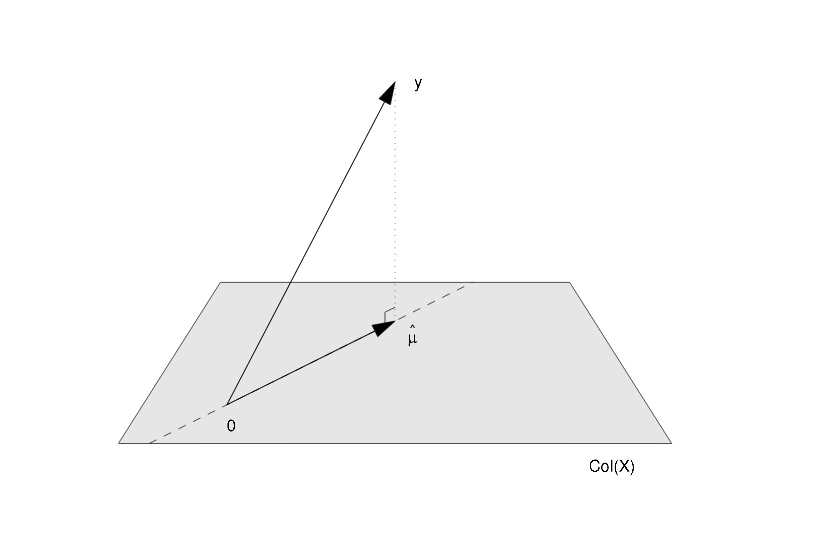
\includegraphics[scale=0.4]{Immagini/spazio-col.png}
\caption{Rappresentazione dello spazio delle colonne e dei vettori di interesse.}
\end{figure}

La bontà di adattamento si stima in base a \textit{devianza totale} e
\textit{devianza spiegata}.\\
La \textit{devianza spiegata} è la somma delle differenze al quadrato tra i valori teorici della retta interpolante e la media dei valori empirici.\\
La \textit{devianza residua} è la somma degli scarti al quadrato tra i valori osservati e teorici della $y$. \\
La \textit{devianza totale} è la somma degli scarti dei valori di $y$ empirici dalla loro media.

L'indice di adattamento è definito come:
\begin{equation}
R^2 = \frac{DevSpieg(Y)}{DevTot(Y)}
\end{equation}
Nel caso di un modello di regressione lineare semplice si ha che:
\begin{equation}
DevSpieg(Y) = b_1 Codev(X, Y)
\end{equation}
Dividendo per $n-1$ e con opportuni passaggi (si veda http://www2.stat.unibo.it/montanari/Didattica/lab3.pdf) si arriva a:
\begin{equation}
R^2 = \frac{Cov(X, Y)}{var(X)var(Y)}
\end{equation}

$R^2$ è un numero che varia tra 0 e 1, è = 0 se non c'è correlazione lineare, = 1 se c'è perfetta correlazione.

\subsection{Testare i risultati: t-test e F-measure (test di ipotesi)}
Per testare i risultati ottenuti dei parametri si possono effettuare due misure di test sull'ipotesi nulla che il coefficiente stimato sia o meno uguale a zero, ovvero:
\begin{equation}
H_0 = \beta_i = 0
\end{equation}

\begin{tcolorbox}[title = Il test di ipotesi e \textit{p-value}]
Un test di ipotesi è un procedimento tramite il quale si verifica la validità di una certa ipotesi. Solitamente si parte definendo un'\textit{ipotesi nulla} tramite la quale si afferma che per la popolazione, o comunque più in generale per il fenomeno che si sta studiando, vale una determinata condizione, ovvero:
\begin{equation}
H_0 = \mu 
\end{equation}
dove $\mu$ sta a indicare una qualsiasi condizione che si vuole testare. \\
L'\textit{ipotesi alternativa} invece specifica che cosa è vero nel caso in cui l'ipotesi nulla sia falsa. La più generale ipotesi alternativa è il contrario dell'ipotesi nulla ovvero:
\begin{equation}
H_1 \neq \mu 
\end{equation}
La valutazione dei risultati di un test di ipotesi avviene considerando il cosiddetto \textit{p-value}. Per calcolare il p-value si calcola prima la distribuzione di probabilità per l'ipotesi nulla, assumendo quindi che essa sia vera, ed in seguito per calcolare il p-value bisogna calcolare la probabilità di ottenere un valore che sia più grande del valore osservato. Quindi l'area sottesa alla parte di curva a destra del valore osservato.\\
FIGURAAAA
Vogliamo che la probabilità evidenziata sia la più piccola possibile, ovvero che il valore osservato sia il più possibile discostato dal centro della curva in quanto essa è centrata sull'ipotesi nulla.\\
Se stabiliamo un livello di confidenza $\alpha$ ciò significa che la \textit{probabilità} di ottenere un valore uguale o più grande del valore osservato deve essere minore o uguale a $\alpha$. Quindi la parte di curva (probabilità) dentro le regioni delle code esterne individuate da $\alpha$ è uguale a $1-\alpha$.
\begin{equation}
P(-Z_{\frac{\alpha}{2}}< a < +Z_{\frac{\alpha}{2}}) = 1 - \alpha
\end{equation}
Dove $-Z_{\frac{\alpha}{2}}$ e $+Z_{\frac{\alpha}{2}}$ rappresentano i valori di $a$ tali per cui la probabilità racchiusa all'interno di questi valori è uguale a $1-\alpha$. Se standardizziamo la distribuzione della quantità $a$ in modo da renderla a media nulla e varianza 1 (quindi sottraiamo la media e dividiamo per la deviazione standard), otteniamo:
\begin{equation}
P(-Z'_{\frac{\alpha}{2}}< \frac{a - \mu_a(H_0)}{\sigma} < +Z'_{\frac{\alpha}{2}}) = 1 - \alpha
\end{equation}
che implica che $a$ deve trovarsi entro i seguenti valori in termini di deviazione standard rispetto alla media:
\begin{equation}
\label{eq: prob-interna}
P(\mu_a(H_0) - Z'_{\frac{\alpha}{2}} \cdot \sigma < a < \mu_a(H_0) + Z'_{\frac{\alpha}{2}} \cdot \sigma) = 1 - \alpha
\end{equation}
I valori di $Z'$ sono tabulati dalla funzione degli errori.\\
La probabilità (p-value) per un valore osservato di $a$ è:
\begin{equation}
p = P( \vert \frac{a - \mu_a(H_0)}{\sigma} \vert > \vert \frac{a_{oss} - \mu_a(H_0)}{\sigma} \vert)
\end{equation}
che rappresenta quindi la probabilità di osservare un valore di $a$ maggiore o uguale a quello che si è osservato (supponendo valida l'ipotesi nulla). Se questo valore di probabilità è inferiore al livello $\alpha$ fissato (quindi il valore $a_{oss}$ è al di fuori dell'intervallo individuato in termini di $Z'$ intervalli di confidenza) si può rigettare l'ipotesi nulla.
\end{tcolorbox}

\subsubsection{t-test}

La \textit{t-statistic}, detta anche \textit{t-measure} o \textit{t-test}, rappresenta un modo per valutare se la stima di una quantità risulta accettabile o meno rispetto ad un'ipotesi nulla. È definita come segue:
\begin{equation}
t = \frac{a - a_0}{SE(a)}
\end{equation}
dove $a_0$ è il valore dell'ipotesi nulla che si sta testando per la quantità $a$ e $SE$  è lo \textit{standard error} di questa variabile ovvero: $\frac{\sigma}{\sqrt{n}}$.\\
Quindi nel caso della stima dei parametri $\beta$ della regressione lineare semplice, in cui per l'ipotesi nulla si suppone che $\beta$ abbia valore zero,  si ha:
\begin{equation}
t = \frac{\beta_i}{SE(\beta_i)} = \frac{\beta_i}{\frac{\sigma}{\sqrt{n \sigma_{jj}}}}
\end{equation}
se la $\sigma$ è nota, altrimenti si usa il suo stimatore $s$, quindi:
\begin{equation}
t = \frac{\beta_i}{\frac{s}{\sqrt{n \sigma_{jj}}}}
\end{equation}
Se si fissa quindi un livello di confidenza $\alpha$ per il p-value,  per esempio $\alpha = 0,05$, si ottiene che l'ipotesi nulla deve essere rigettata se $t > 1,96$. \\
Si può quindi riscrivere il p-value in termini della statistica t:
\begin{equation}
p = P(t > t_{oss})
\end{equation}

Se la quantità $a$ è distribuita normalemnte allora t è distribuito come un $\chi^2$ a $n-1$ gradi di libertà che tende ad una distribuzione normale per grandi $n$ (si veda Stock p.87).
\subsubsection{F measure}
Nel caso sia condotta una regressione con più regressori si può effettuare un test di ipotesi congiunto per i vari parametri che vengono stimati, ovvero vedere se un determinato set di parametri è efficiente o meno nella stima del modello. Quindi è definita la seguente ipotesi nulla:
\begin{equation}
\begin{split}
H_0 &: \; \beta_0 = 0 ,\; \beta_1 = 0,\; \cdot ,\; \beta_k = 0 \\
&:\; \beta_0 =  \beta_1 = \cdot = \beta_k = 0
\end{equation}
che implica l'ipotesi alternativa:
\begin{equation}
H_1: \; \beta_0 \neq 0 ,\; \beta_1 \neq 0,\; \cdot ,\; \beta_k \neq 0
\end{equation}
ovvero si testa se uno tra i parametri stimati sia nullo, se si rifiuta l'ipotesi nulla significa che almeno uno di essi non è nullo, e quindi è significativo.

Il test di ipotesi congiunta si effettua calcolando la F-measure per il modello lineare preso in esame, definita come segue:
\begin{equation}
F = \frac{SSR_r - SSR_{ur}/q}{SSR_{ur}/(n-(k+1))}
\label{F-measure}
\end{equation}
dove $SSR$ rappresenta la somma dei residui al quadrato del modello, cioè la devianza residua. In particolare $SSR_r$ rappresenta la devianza residua per il modello ristretto all'ipotesi nulla, ovvero, supponendo vera l'ipotesi nulla, $SSR_r$ rappresenta la devianza residua del modello in cui i parametri sono posti uguale ai valori specificati dall'ipotesi, in questo caso sono posti uguale a zero. $SSR_{ur}$ rappresenta invece la devianza residua per il modello non ristretto, ovvero quello stimato con tutti i parametri. La variabile $q$ rappresenta invece il numero di restrizioni, ovvero il numero di parametri che sono testati congiuntamente, $n$ rappresenta il numero di osservazioni e $k$ il numero di variabili indipendenti nel modello non ristretto. Le due quantità rapportate nell'equazione \eqref{F-measure} sono distribuite come un $\chi^2$ che implica che la $F$ sia distribuita come una F di Fisher-Snedecor con $q$ e $n-(k+1)$ gradi di libertà. Possiamo quindi impostare un livello di significatività $\alpha$ con il quale rifiutare l'ipotesi nulla. L'ipotesi nulla è accettata se:
\begin{equation}
P(F_0 < F_\alpha) = 1-\alpha
\end{equation}
ovvero se si ottiene un valore per il test $F_0$ minore del valore $F_\alpha$, valore per cui la probabilità è uguale a $1-\alpha$. Questo valore si può trovare tabulato. Se invece si trova un valore maggiore, tale per cui la probabilità di ottenere un valore maggiore o uguale è uguale o minore di $\alpha$, allora si può rigettare l'ipotesi nulla.
\section{Regressione logistica}
[ref: https://codesachin.wordpress.com/2015/08/16/logistic-regression-for-dummies/ , https://www.youtube.com/watch?v=gNhogKJ\_q7U]\\
La regressione logistica a differenza di altri tipi di regressione non si pone l'obiettivo di predire il valore di una variabile dato un certo numero di input. La regressione logistica si applica infatti a variabili categoriche. La regressione logistica restituisce in output la \textit{probabilità} che un certo punto in input appartenga ad una certa classe. Assumiamo per semplicità di avere solamente due classi (classe binaria) in cui la variabile dipendente $y$ può assumere valori. A differenza della regressione lineare classica quindi la variabile dipendente può assumere solamente un numero finito di valori e non uno spettro continuo. Possiamo comunque provare ad applicare una regressione lineare ad un problema che coinvolge variabili questo tipo, infatti a parte essere una variabile binaria, non c'è nulla di speciale nella variabile y che vogliamo prevedere, i problemi sorgono quando si devono poi interpretare i risultati restituiti da questo modello. Applichiamo quindi un modello lineare utilizzando tutte le variabili indipendenti $x_1, \cdots, x_n$ che si ritengono significative per la previsione di un'uscita della variabile $y$. Sia questa uscita $y=1$, più il risultato restituito dal modello, per determinati valori delle variabili indipendenti, è alto, più sarà probabile che il valore per la variabile dipendente sia effettivamente uguale a $1$. Per esempio possiamo considerare il caso di superare o meno un esame, la possibilità di successo la codifichiamo con il valore $y=1$, mentre quella di insuccesso con il valore $y=0$. Per convenzione solitamente si predice la variabile che viene indicata con $1$, quindi in questo caso la possibilità di successo, di conseguenza inseriamo nel modello tutte quelle variabili che riteniamo significative per questa predizione. Supponendo di avere tra le variabili solamente il tempo di studio il modello lineare avrà la seguente forma:
\begin{equation}
y = \beta_0 + \beta_1\cdot tempo\;di\;studio
\label{eq: esempio-regressione-lineare-logistica}
\end{equation}
dai risultati di questa predizione otterremo dei valori per i coefficienti che vengono stimati tramite maximum likelihood (per approfondire si veda https://onlinecourses.science.psu.edu/stat504/node/150) ma cosa significa il risultato di questa regressione. Supponiamo per esempio di ottenere come risultati $\beta_0 = -1$ e $\beta_1 = 2$, se consideriamo un tempo di studio pari a 2 ore e lo inseriamo all'interno dell'equazione otteniamo per la variabile $y$, che in questo caso rappresenta la possibilità di superare l'esame, un valore pari a 1, ma cosa indica? Così com'è per ora non indica nulla, infatti se volessimo interpretarlo come la probabilità di superare l'esame sbaglieremmo in quanto quest'ultima deve sempre risiedere tra 0 e 1, mentre in questo caso se per esempio consideriamo un tempo di studio di 5 ore per esempio otteniamo un valore negativo, e se scegliamo il caso in cui il tempo di studio sia nullo si ottiene per $y$ un risultato negativo. Per poter passare dai risultati della regressione lineare a delle probabilità $P$ è necessario applicare una trasformazione non lineare che:
\begin{enumerate}
\item Assuma sempre valori positivi
\item Sia compresa tra 0 e 1
\end{enumerate} 
Per soddisfare il primo punto si applica una funzione esponenziale all'espressione della regressione lineare quindi dalla \eqref{eq: esempio-regressione-lineare-logistica}, che più in generale può essere riscritta come $y = \beta_0 + \beta_1 \cdot x_1 + \beta_2 \cdot x_2 + \cdots$, si passa a:
\begin{equation}
P = \exp(\beta_0 + \beta_1 \cdot x_1 + \beta_2 \cdot x_2 + \cdots)
\end{equation}
Ora è necessario che $P$ sia compresa risulti minore di $1$, in quanto con il passaggio precedente ci assicuriamo già che assuma solo valori positivi. Per fare ciò ci basta divider l'espressione precedentemente ricavata per un numero che sia leggermente più grande, di modo da ottenere così una funzione che tenda asintoticamente a $1$ e a $0$. Per fare questo dividiamo per la stessa quantità a cui sommiamo $1$, ottenendo così l'espressione per la probabilità:
\begin{equation}
P = \frac{\exp(y = \beta_0 + \beta_1 \cdot x_1 + \beta_2 \cdot x_2 + \cdots)}{\exp(y = \beta_0 + \beta_1 \cdot x_1 + \beta_2 \cdot x_2 + \cdots) + 1}
\end{equation}
L'interpretazione del modello lineare si può però ancora mantenere in quanto:
\begin{equation}
\log(\frac{P}{1-P}) = \beta_0 + \beta_1 \cdot x_1 + \beta_2 \cdot x_2 + \cdots
\label{eq: logit}
\end{equation}
dove $1-P$ oltre a permettere il passaggio per ottenere l'espressione lineare, dal punto di vista interpretativo rappresenta la probabilità di ottenere $y = 0$. A volta ci si riferisce al rapporto $\frac{P}{1-P}=\frac{P(y=1)}{P(y=0)}$ con il termine di \textit{Odds ratio}. Quando viene applicata la regressione logistica viene applicata la formula \eqref{eq: logit}, detta anche \textit{logit}, per cui per ottenere i valori di probabilità associati a determinati valori delle variabili indipendenti che si sono utilizzate è necessario applicare la formula inversa.
nei software è spesso anche possibile impostare una soglia per la probabilità con la qual stabilire e quindi predire se una certa osservazione con una certa probabilità appartenga ad una determinata classe. In questo modo si possono poi calcolare delle contingency table dalle quali vedere quanti valori sono stati correttamente predetti e quanti invece no.

\section{Violazioni del modello lineare classico}

\subsection{Eteroschedasticità}
L'ipotesi di omoschedasticità suppone che il termine di errore sia uguale per tutte le variabili indipendenti. Però ci possono essere situazioni in cui ciò non è vero, ovvero situazioni in cui il termine di errore varia tra le diverse variabili indipendenti,  in questo caso se osserviamo uno scatter plot dei residui in funzione dei valori predetti per la variabile dipendente osserviamo un tipico andamento a cono. Un altro andamento anomalo di qeusto tipo lo si può osservare in un semplice grafico scatter plot della variabile dipendente in funzione della variabile indipendente. nel caso di errori omoschedastici i punti sono collocati in modo equidistante dalla retta interpolante, mentre nel caso di errori eteroschedastici i punti sono distanziati in maniera diversa da questa. Il problema nel caso eteroschedastico si pone in quanto il metodo OLS (Ordinary Least Squares) cioè il metodo dei minimi quadrati ordinari mira a minimizzare i residui ottenendo lo standard error minimo. Il metodo OLS pesa però tutte le osservazioni allo stesso modo, mentre quando si trattano errori eteroschedastici è necessario pesare meno i valori con più errore e pesare di più quelli che invece sono più rilevanti.\\
Se utilizziamo ancora stimatori OLS cosa succede?\\
Valgono ancora le ipotesi di correttezza e linearità.\\
È ancora consistente.\\
Non è più uno stimatore\\
In 	questo caso lo stimatore non è più efficiente.

La statistica t di Student non può approssimare nel modo corretto la varianza $\sigma^2$ per due ragioni:
\begin{enumerate}
\item le stime campionare tendono a sottostimare il valore della varianza
\item non c'è più da calcolare una sola varianza ma diverse varianze.
\end{enumerate}

Come conseguenza della sottostima della varianza si ha che la statistica t di Student ha valori erroneamente elevati, si possono considerare come significativi paramentri che in realtà non lo sono. Per lo stesso motivo la regione di accettazione diventa molto più piccola di quanto non lo sia in realtà e di conseguenza la regione di rifiuto molto grande.

L'ipotesi di omoschedasticità (uguali varianze) è alla base di test come l'analisi della varianza ANOVA (Analysis Of Variance) e il t-test di Student.

Oltre alla visualizzazione grafiche, l'eteroschedasticità si può individuare anche tramite metodi analitici, ovvero eseguendo dei test come il \textit{test di White} o il \textit{test di Breuch-Pagan}.





\end{document}
